\clearpage
\section{Numerical fitting and residual comparisons}
\label{sec:fits}
\subsection{Exactly which data enter each fit}
\label{sec:fit-selection}
Both models use the 105-geometry grid in Eq.~\eqref{eq:large-grid},
with six ordered pairs, giving 630 values per model. The fitting and
display windows in Eq.~\eqref{eq:fit-display-windows} give
\begin{center}
\begin{tabular}{rll}\toprule
$N$ & Fitted $\ell$ ($x\leq0.08$) & Displayed $\ell$ ($x\leq0.20$)\\\midrule
32&none&4, 5, 6\\
48&none&4, 5, 6, 7, 8, 9\\
64&4, 5&4--10\\
82&4, 5, 6&4--10\\
96&4, 5, 6, 7&4--10\\
112&4, 5, 6, 7, 8&4--10\\
128,144,160,176&4--10 each&4--10 each\\
192,208,224,240,256&4--10 each&4--10 each\\\bottomrule
\end{tabular}
\end{center}
Every directional fit uses exactly $m=77$ samples from 13 sizes, and
every model comparison uses those same samples. Every figure panel
shows 100 samples, including 23 excluded from fitting. No point lies
exactly at either cutoff: the largest fitted value is $5/64=0.078125$, and
the largest displayed value is $6/32=9/48=0.1875$. There is
no averaging of reverse directions or points with the same $x$.
The Ising production set consists of exact finite-chain states for all 15
sizes; the pure-block and puMPS comparisons in Appendix~\ref{sec:state-comparisons}
validate its relationship to the requested construction. Historical
one-site observations remain archived and are excluded from the present
fits. The boson uses the same finite-$W$ state, with the contraction
and precision controls in Sec.~\ref{sec:extension}.

\subsection{Ansatz, objective function, and every reported indicator}
For a finite truncation of Eq.~\eqref{eq:hierarchy}, define
\begin{equation}
 F_K(x;\bm c)=\sum_{j=0}^{K-1}c_{\alpha+2j}(\pi x)^{\alpha+2j},
 \quad K=1,2,3,4.
 \label{eq:fit}
\end{equation}
All $K$ coefficients are free and optimized jointly. The leading exponent
$\alpha$ is fixed by the theory; subsequent exponents are fixed to the
consecutive even powers assumed in Eq.~\eqref{eq:hierarchy}.
No exponent is optimized, and the leading coefficient is not held at its
theoretical value. This is a numerical coefficient estimate, not an
analytic derivation of subleading coefficients.
There is no constant term. The leading-only comparison is $F_1$; the
primary corrected comparison is $F_3$. Thus $F_3$ contains $x^2,x^4,x^6$
for ten directions and $x^4,x^6,x^8$ for $I\leftrightarrow\eps$.
The last coefficient is fitted even when its analytic value is unknown.
Tables in Appendix~\ref{sec:allfits} also show $F_2$ and $F_4$, which
include all assumed even powers through $\alpha+2$ and $\alpha+6$, respectively.
All four truncations are displayed in the fit and residual figures.

Let $y_i$ denote numerical relative entropy at $x_i$ and let
$r_i=y_i-F_K(x_i)$. The ordinary, unweighted, linear least-squares
problem is
\begin{equation}
 \widehat{\bm c}=\arg\min_{\bm c}\sum_{i=1}^{m}r_i^2,\qquad m=77,
 \quad x_i\leq0.08.
 \label{eq:objective}
\end{equation}
It is fitted in $D$ itself, not its logarithm; data are deterministic
contractions, so no sampling-error weights are assumed. To stabilize the
design matrix, the solver uses $X_{ij}=(x_i/0.08)^{\alpha+2j}$,
then converts its coefficients to the $(\pi x)$ convention.
The stored condition number is $\kappa_X=s_{\max}(X)/s_{\min}(X)$, the
ratio of extreme singular values of this scaled matrix.

We report the following quantities explicitly:
\begin{align}
 \mathrm{SSE}&=\sum_i r_i^2,
 &\mathrm{RMSE}&=\sqrt{\mathrm{SSE}/m},
 &r_{\max}&=\max_i|r_i|,\notag\\
 \mathrm{RMSrel}\,[\%]&=100\sqrt{\frac1m\sum_i(r_i/y_i)^2},
 &\mathrm{MAPE}\,[\%]&=\frac{100}m\sum_i|r_i/y_i|,\notag\\
 G_K[\%]&=100\left(1-\frac{\mathrm{RMSE}_K}{\mathrm{RMSE}_1}\right),
 &\delta c_\alpha[\%]&=100\left(\frac{\widehat c_\alpha}{c_\alpha^{\rm CFT}}-1\right).
 \label{eq:metrics}
\end{align}
The residual plots show the signed percentage $100r_i/y_i$ on the
larger display window. All metrics in Eq.~\eqref{eq:metrics}, the
standard errors and the cross-validation scores use only $x_i\leq0.08$.
The 23 displayed points outside that cutoff test extrapolation of the
same fitted coefficients and never enter the optimization.
A positive gain $G_K$ means a reduction in root-mean-square residual, not
a percentage change of SSE. The fitted model has $k=K$ free parameters
and $m-k$ residual degrees of freedom. The CSV also stores descriptive
ordinary-least-squares standard errors from
$(\mathrm{SSE}/(m-k))(X^TX)^{-1}$, converted with the same column scaling.
These errors are not statistical confidence intervals: they do not account
for systematic finite-lattice effects or truncation of the continuum series.

To test whether extra terms predict another size, leave out one complete
chain length $N$ at a time, refit to the other 12 contributing sizes, and denote the
predicted value by $F_K^{(-N_i)}(x_i)$. Define
\begin{equation}
 \mathrm{CVRMSE}_K=\sqrt{\frac1m\sum_i
 [y_i-F_K^{(-N_i)}(x_i)]^2},\quad
 G_K^{\rm CV}[\%]=100\left(1-\frac{\mathrm{CVRMSE}_K}{\mathrm{CVRMSE}_1}\right).
 \label{eq:cv}
\end{equation}
The superscript CV means cross-validation. The tables also report the
minimum and maximum leading coefficient across these 13 refits, denoted
$c_\alpha^{\rm LOO,min/max}$ (LOO means leave one size out).
With no noise model or controlled continuum extrapolation, this variation is more
informative than nominal coefficient significance.

For comparison with the numerical fits, ``CFT'' means the analytical CFT
series supplied by the original paper in Sec.~\ref{sec:coefficients},
with zero free parameters. For bosons and the four Ising spin channels,
it includes only power $2$. For the two Ising identity--energy channels,
it includes powers $4,6$. Unavailable coefficients are omitted from this
comparison, not asserted to vanish.
The CFT row's CV RMSE equals its RMSE because there is nothing to refit.

\subsection{Results and limitations of a fit depending only on \texorpdfstring{$x$}{x}}
\begin{table}[p]\centering\scriptsize
\begin{tabular}{llrrrrrr}\toprule
Direction & Fit & $c_{\alpha}$ & $c_{\alpha+2}$ & $c_{\alpha+4}$ & RMSE & Gain (\%) & CV RMSE\\\midrule
$I\mid \sigma$ & $F_1$ & 0.020884 & -- & -- & $4.46\!\times\!10^{-7}$ & 0.0 & $4.84\!\times\!10^{-7}$ \\
$I\mid \sigma$ & $F_3$ & 0.020856 & $4.29\!\times\!10^{-4}$ & 0.0062415 & $2.95\!\times\!10^{-7}$ & 33.8 & $3.56\!\times\!10^{-7}$ \\
\addlinespace[2pt]
$\sigma\mid I$ & $F_1$ & 0.02088 & -- & -- & $3.69\!\times\!10^{-7}$ & 0.0 & $3.96\!\times\!10^{-7}$ \\
$\sigma\mid I$ & $F_3$ & 0.020852 & $4.92\!\times\!10^{-4}$ & 0.0048452 & $1.86\!\times\!10^{-7}$ & 49.5 & $2.23\!\times\!10^{-7}$ \\
\addlinespace[2pt]
$I\mid \varepsilon$ & $F_1$ & 0.12424 & -- & -- & $1.90\!\times\!10^{-6}$ & 0.0 & $2.09\!\times\!10^{-6}$ \\
$I\mid \varepsilon$ & $F_3$ & 0.13058 & -0.10453 & -0.49319 & $8.22\!\times\!10^{-7}$ & 56.7 & $1.14\!\times\!10^{-6}$ \\
\addlinespace[2pt]
$\varepsilon\mid I$ & $F_1$ & 0.11711 & -- & -- & $3.16\!\times\!10^{-6}$ & 0.0 & $3.39\!\times\!10^{-6}$ \\
$\varepsilon\mid I$ & $F_3$ & 0.13044 & -0.28536 & 0.23803 & $7.53\!\times\!10^{-7}$ & 76.2 & $1.03\!\times\!10^{-6}$ \\
\addlinespace[2pt]
$\sigma\mid \varepsilon$ & $F_1$ & 0.025634 & -- & -- & $4.40\!\times\!10^{-5}$ & 0.0 & $4.57\!\times\!10^{-5}$ \\
$\sigma\mid \varepsilon$ & $F_3$ & 0.020772 & 0.13303 & -0.2023 & $2.46\!\times\!10^{-6}$ & 94.4 & $3.08\!\times\!10^{-6}$ \\
\addlinespace[2pt]
$\varepsilon\mid \sigma$ & $F_1$ & 0.024168 & -- & -- & $2.94\!\times\!10^{-5}$ & 0.0 & $3.05\!\times\!10^{-5}$ \\
$\varepsilon\mid \sigma$ & $F_3$ & 0.020785 & 0.097933 & -0.26034 & $2.85\!\times\!10^{-6}$ & 90.3 & $3.63\!\times\!10^{-6}$ \\
\addlinespace[2pt]
\bottomrule\end{tabular}

\caption{Ising leading-only ($F_1$, $k=1$) and three-term ($F_3$, $k=3$)
fits to the same 77 points selected from Eq.~\eqref{eq:large-grid}
by $x\leq0.08$, with $p=1/2$ and critical Hamiltonian~\eqref{eq:Hising}.
Section~\ref{sec:fit-selection} specifies every contributing size and interval.
The coefficients multiply $(\pi x)^r$; $\alpha=4$ for
$I\leftrightarrow\eps$ and two otherwise. The degrees of freedom are
76 and 74. RMSE and CV RMSE are in nats; Gain is $G_K$ from
Eq.~\eqref{eq:metrics}. No coefficient is fixed to its CFT value.}
\label{tab:isingfits}
\end{table}
\begin{table}[p]\centering\scriptsize
\begin{tabular}{llrrrrrr}\toprule
Direction & Fit & $c_{\alpha}$ & $c_{\alpha+2}$ & $c_{\alpha+4}$ & RMSE & Gain (\%) & CV RMSE\\\midrule
$00\mid ss$ & $F_1$ & 0.078322 & -- & -- & $4.02\!\times\!10^{-5}$ & 0.0 & $4.34\!\times\!10^{-5}$ \\
$00\mid ss$ & $F_3$ & 0.076917 & 0.082853 & -1.045 & $3.97\!\times\!10^{-5}$ & 1.1 & $4.81\!\times\!10^{-5}$ \\
\addlinespace[2pt]
$ss\mid 00$ & $F_1$ & 0.078327 & -- & -- & $4.01\!\times\!10^{-5}$ & 0.0 & $4.33\!\times\!10^{-5}$ \\
$ss\mid 00$ & $F_3$ & 0.076919 & 0.082763 & -1.0418 & $3.97\!\times\!10^{-5}$ & 1.1 & $4.80\!\times\!10^{-5}$ \\
\addlinespace[2pt]
$00\mid 3s,s$ & $F_1$ & 0.39311 & -- & -- & $1.64\!\times\!10^{-4}$ & 0.0 & $1.78\!\times\!10^{-4}$ \\
$00\mid 3s,s$ & $F_3$ & 0.39364 & 0.16385 & -3.9364 & $1.55\!\times\!10^{-4}$ & 5.3 & $1.86\!\times\!10^{-4}$ \\
\addlinespace[2pt]
$3s,s\mid 00$ & $F_1$ & 0.39342 & -- & -- & $1.58\!\times\!10^{-4}$ & 0.0 & $1.72\!\times\!10^{-4}$ \\
$3s,s\mid 00$ & $F_3$ & 0.39376 & 0.16408 & -3.8368 & $1.50\!\times\!10^{-4}$ & 5.1 & $1.79\!\times\!10^{-4}$ \\
\addlinespace[2pt]
$ss\mid 3s,s$ & $F_1$ & 0.16341 & -- & -- & $4.06\!\times\!10^{-5}$ & 0.0 & $4.39\!\times\!10^{-5}$ \\
$ss\mid 3s,s$ & $F_3$ & 0.1628 & 0.060263 & -0.99798 & $3.98\!\times\!10^{-5}$ & 1.7 & $4.71\!\times\!10^{-5}$ \\
\addlinespace[2pt]
$3s,s\mid ss$ & $F_1$ & 0.1636 & -- & -- & $3.72\!\times\!10^{-5}$ & 0.0 & $4.01\!\times\!10^{-5}$ \\
$3s,s\mid ss$ & $F_3$ & 0.16288 & 0.06078 & -0.9399 & $3.67\!\times\!10^{-5}$ & 1.4 & $4.29\!\times\!10^{-5}$ \\
\addlinespace[2pt]
\bottomrule\end{tabular}

\caption{Boson fits with the same geometries, probability, objective, and
parameter counts as Table~\ref{tab:isingfits}; $\alpha=2$ for every row.
States use charge codes $(0,0),(1,1),(3,1)$, lattice exponent $q=2$,
unit-circle coordinates, $w_1=0$, $W=w_2=10^8$, no orthogonalization,
and natural logarithms. All coefficients multiply powers of $\pi x$.
Gain compares training RMSE with the free-coefficient leading-only fit.}
\label{tab:bosonfits}
\end{table}

Training RMSE decreases by $33.8$--$94.4\%$ in Ising and
$1.11$--$5.31\%$ in the boson. Since $F_1$ is nested in $F_3$, some
training improvement is automatic. Cross-validation is more selective:
all six boson directions have negative CV gain, from $-10.8\%$ to
$-4.20\%$, while all six Ising directions
improve by $26.4$--$93.3\%$. Adding still more powers is therefore not a
universal remedy for this data window.

The $F_3$ leading-coefficient errors are $-7.70\%$ to $-2.27\%$ for the
boson and $-2.17\%$ to $+0.11\%$ for Ising.
For $\sigma\mid\eps$, the fitted $c_2=0.020772$ differs from $1/48$
by $-0.296\%$. Appendix~\ref{sec:window-comparison} compares the
$x\leq0.20$, $0.12$, and $0.08$ fits on the same computed grid.
A small residual alone does not establish the continuum coefficient:
finite-interval lattice effects remain even for exact eigenstates.

\begin{table}[p]\centering\scriptsize
\begin{tabular}{lrrrrrr}\toprule
Direction & $\delta c_\alpha$ (\%) & RMS rel. (\%) & Max $|r|$ & CV gain (\%) & $c_\alpha^{\rm LOO,min}$ & $c_\alpha^{\rm LOO,max}$\\\midrule
$I\mid \sigma$ & 0.11 & 0.06 & $1.48\!\times\!10^{-6}$ & 26.4 & 0.020852 & 0.020859 \\
$\sigma\mid I$ & 0.09 & 0.04 & $8.77\!\times\!10^{-7}$ & 43.7 & 0.020849 & 0.020854 \\
$I\mid \varepsilon$ & -2.06 & 0.79 & $3.90\!\times\!10^{-6}$ & 45.6 & 0.12944 & 0.13192 \\
$\varepsilon\mid I$ & -2.17 & 0.77 & $3.60\!\times\!10^{-6}$ & 69.5 & 0.12944 & 0.13164 \\
$\sigma\mid \varepsilon$ & -0.30 & 0.31 & $1.29\!\times\!10^{-5}$ & 93.3 & 0.020734 & 0.020806 \\
$\varepsilon\mid \sigma$ & -0.23 & 0.35 & $1.46\!\times\!10^{-5}$ & 88.1 & 0.020733 & 0.020833 \\
\bottomrule\end{tabular}

\caption{Diagnostics for the Ising $F_3$ fits of
Table~\ref{tab:isingfits}. Signed leading-coefficient errors, RMS relative
residuals, maximum absolute residuals (nats), CV gain, and extrema of the
13 leave-one-size-out leading coefficients follow
Eqs.~\eqref{eq:metrics}--\eqref{eq:cv}. These extrema are sensitivity
measures, not confidence bounds.}
\end{table}
\begin{table}[p]\centering\scriptsize
\begin{tabular}{lrrrrrr}\toprule
Direction & $\delta c_\alpha$ (\%) & RMS rel. (\%) & Max $|r|$ & CV gain (\%) & $c_\alpha^{\rm LOO,min}$ & $c_\alpha^{\rm LOO,max}$\\\midrule
$00\mid ss$ & -7.70 & 2.36 & $1.72\!\times\!10^{-4}$ & -10.8 & 0.076448 & 0.077586 \\
$ss\mid 00$ & -7.70 & 2.36 & $1.72\!\times\!10^{-4}$ & -10.8 & 0.076453 & 0.077587 \\
$00\mid 3s,s$ & -5.53 & 1.87 & $6.93\!\times\!10^{-4}$ & -4.2 & 0.39201 & 0.39619 \\
$3s,s\mid 00$ & -5.50 & 1.84 & $6.69\!\times\!10^{-4}$ & -4.2 & 0.39225 & 0.39624 \\
$ss\mid 3s,s$ & -2.32 & 1.20 & $1.94\!\times\!10^{-4}$ & -7.1 & 0.16248 & 0.1634 \\
$3s,s\mid ss$ & -2.27 & 1.16 & $1.77\!\times\!10^{-4}$ & -6.9 & 0.16258 & 0.16343 \\
\bottomrule\end{tabular}

\caption{The same diagnostics for the boson $F_3$ fits of
Table~\ref{tab:bosonfits}, with exactly the same fitting window and
indicator definitions. Reverse directions are fitted independently.}
\end{table}

The intervals still contain only four to ten sites; dependence on $N$
and $\ell$ separately limits the continuum comparison. No lattice-correction
law or controlled continuum extrapolation is used.

Extrapolation beyond $x_{\rm fit}=0.08$ can fail. For example, the analytical
CFT truncation~\eqref{eq:epsI} becomes negative for
$x>\sqrt{7/20}/\pi\simeq0.1883$, signaling omitted higher orders since
physical relative entropy is nonnegative. Logarithmic $D$ panels omit
nonpositive predictions; residual panels retain every fitted-polynomial
prediction throughout the displayed window.

\clearpage
\begin{figure}[p]\centering
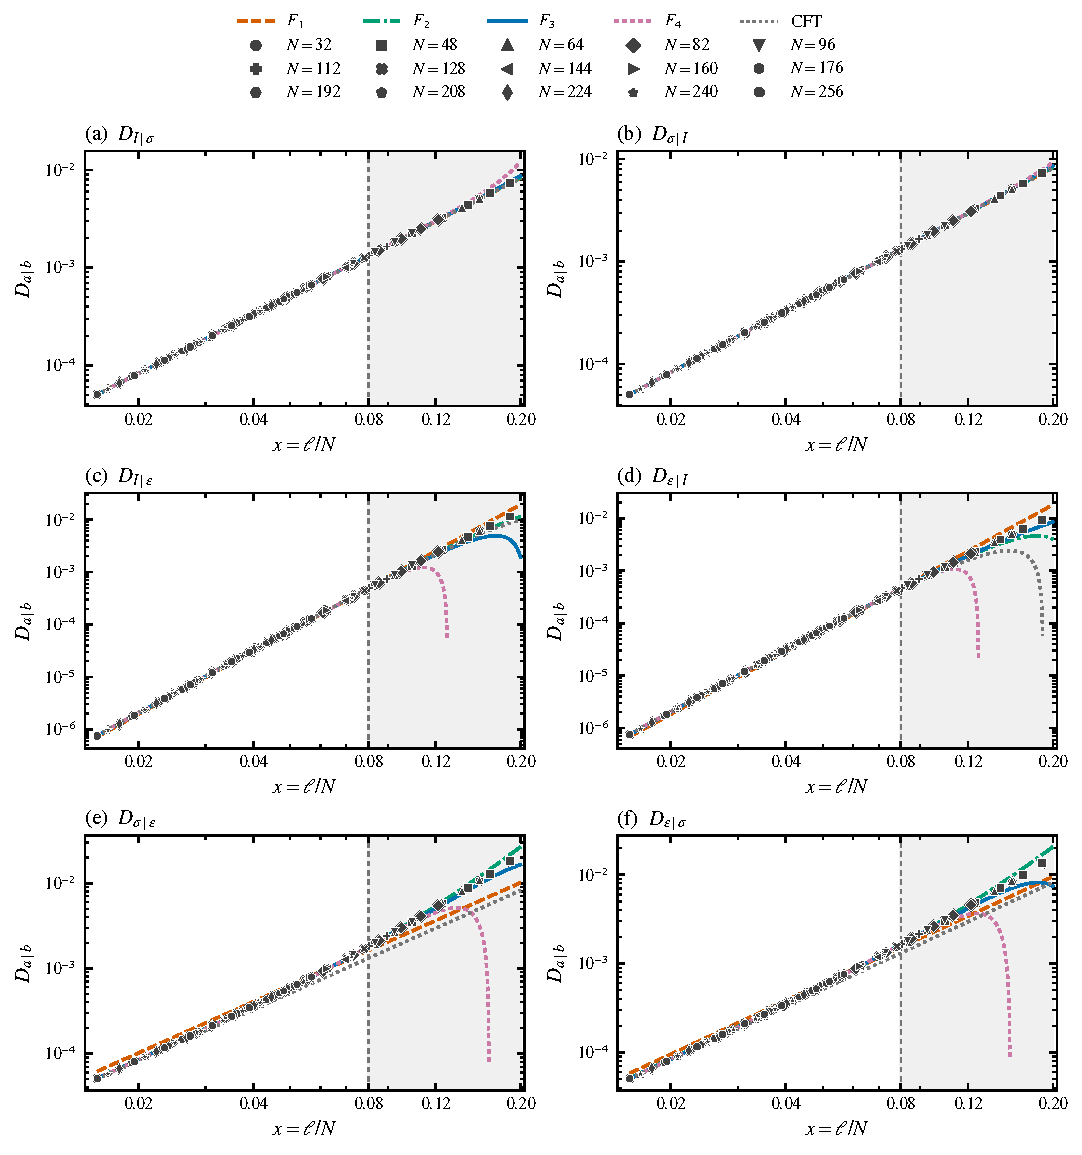
\includegraphics[width=.95\linewidth]{../figs/ising_fits.pdf}
\caption{Ising directed relative entropies at $p=1/2$ in nats.
Each panel displays 100 points from the 15 sizes through $N=256$
in Eq.~\eqref{eq:large-grid}, with $\ell=4,\ldots,10$ and $x\leq0.20$.
Only the 77 points with $x\leq0.08$ determine each fit; the complete
selection is in Sec.~\ref{sec:fit-selection}. The vertical line marks
the fit cutoff, and shading marks the excluded display region.
Both axes are logarithmic to resolve the new small-$x$ observations.
All states belong to the critical periodic-spin Hamiltonian
$H=-\sum XX-\sum Z$; production uses exact Jordan--Wigner interval
matrices, validated against the block states and puMPS as described in
Appendix~\ref{sec:state-comparisons}. Every panel shows
$F_K=\sum_{j=0}^{K-1}c_{\alpha+2j}(\pi x)^{\alpha+2j}$ for $K=1,2,3,4$:
orange dashed $F_1$, green dash--dot $F_2$, blue solid $F_3$, and
purple short-dashed $F_4$. All $K$ coefficients are free; the objective is
unweighted least squares in $D$. The fixed leading exponent is
$\alpha=4$ in panels (c,d) and two otherwise. Gray marker shapes identify
the 15 chain sizes. Dotted gray: the original paper's analytical CFT series (no fitted parameters) through
$x^6$ in (c,d), and its leading $x^2$ term otherwise.
Coefficients, residuals, and fitting conventions are
in Appendix~\ref{sec:allfits} and Eqs.~\eqref{eq:fit}--\eqref{eq:cv};
Table~\ref{tab:isingfits} highlights the $F_1$--$F_3$ comparison.
Curves extend over $1/64\leq x\leq0.20$; beyond the vertical line they
are extrapolations. Nonpositive predictions are omitted on the log axis,
including the analytical CFT truncation in (d) beyond $x\simeq0.1883$.}
\label{fig:isingfits}
\end{figure}
\begin{figure}[p]\centering
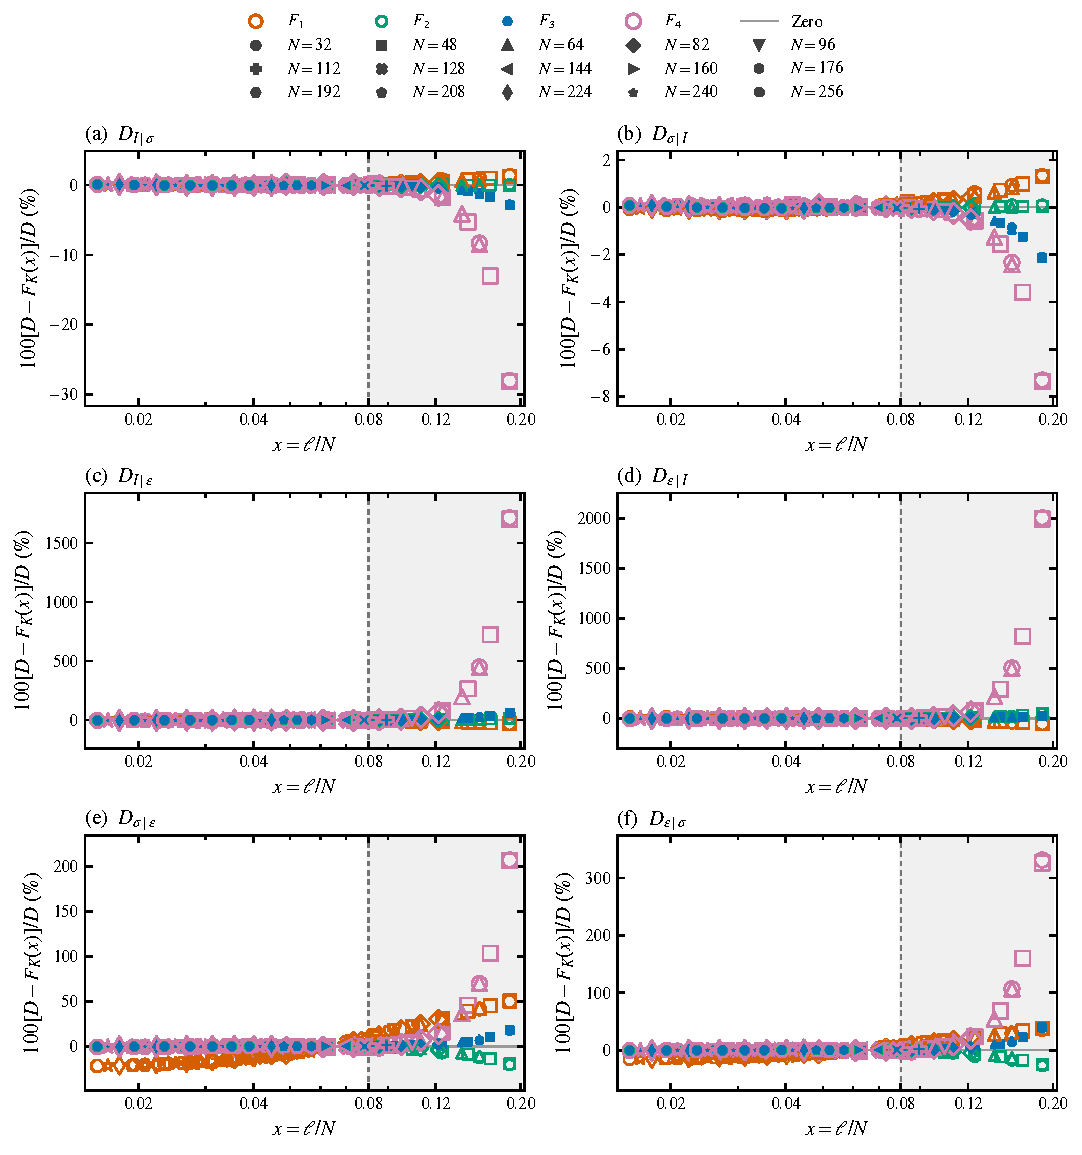
\includegraphics[width=.95\linewidth]{../figs/ising_residuals.pdf}
\caption{Ising residual comparison on exactly the samples and state
parameters of Fig.~\ref{fig:isingfits}. The ordinate is the signed
percentage $100[y_i-F_K(x_i)]/y_i$, where $y_i=D_{a\mid b}(x_i)$.
All four fits are shown: open orange $F_1$, open green $F_2$, filled blue
$F_3$, and open purple $F_4$. Marker shape identifies $N$; marker sizes
differ only to distinguish overlapping series. The horizontal gray line marks zero;
the vertical line and shading identify $x>0.08$, excluded from fitting.
The vertical scale is linear throughout, with ticks showing signed
percentage values directly. The horizontal $x$ axis is logarithmic.
Each $F_K$ has $K$ jointly fitted coefficients at the fixed consecutive
even powers defined in Fig.~\ref{fig:isingfits}. All fits minimize
unweighted squared errors in $D$, not in this percentage.
Appendix~\ref{sec:allfits} gives every fit's coefficients, RMSE, and
leave-one-size-out prediction error. Reduced training residuals alone
do not establish the asymptotic coefficients.}
\label{fig:isingresid}
\end{figure}
\begin{figure}[p]\centering
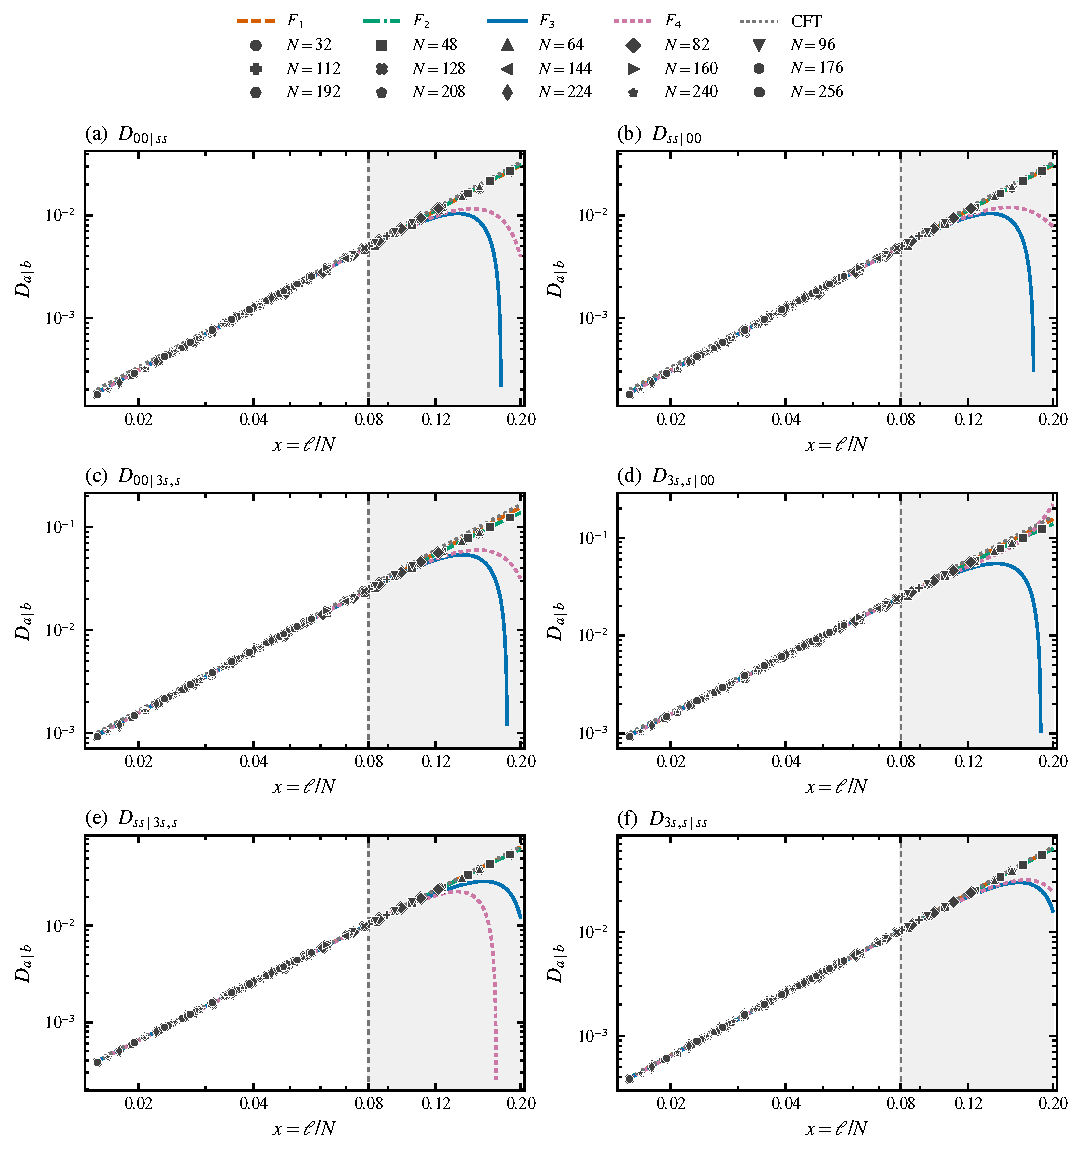
\includegraphics[width=.95\linewidth]{../figs/boson_fits.pdf}
\caption{Boson directed relative entropies at $p=1/2$, natural logarithms,
for charge codes $(0,0),(1,1),(3,1)$, lattice exponent $q=2$,
$z_j=e^{2\pi i j/N}$, $w_1=0$, and $W=w_2=10^8$.
The state generator is Eq.~\eqref{eq:bosonblock}; states are normalized
without orthogonalization. Every panel displays the same 100 geometries
as Fig.~\ref{fig:isingfits}; only the 77 points with $x\leq0.08$ are fitted.
The vertical cutoff line separates fitting from the shaded extrapolation
region through $x=0.20$.
Both axes are logarithmic. The larger-interval state matrices are contracted
by the exact Pfaffian method of Sec.~\ref{sec:extension}, with
100 decimal working digits before conversion to double precision.
Every panel shows $F_K=\sum_{j=0}^{K-1}c_{2+2j}(\pi x)^{2+2j}$,
$K=1,2,3,4$, with $K$ free coefficients and fixed $\alpha=2$.
Orange dashed, green dash--dot, blue solid, and purple short-dashed
curves denote $F_1,F_2,F_3,F_4$, respectively. All fits minimize
unweighted squared errors in $D$; gray marker shapes identify $N$.
Dotted gray: Eq.~\eqref{eq:bosonresult}, with $\kappa=1$ in (a,b),
five in (c,d), and two in (e,f), with no fitted parameter.
Appendix~\ref{sec:allfits} lists all four fits' coefficients and residual
comparisons; Table~\ref{tab:bosonfits} highlights $F_1$ and $F_3$.
Finite-chain reverse directions are retained separately.}
\label{fig:bosonfits}
\end{figure}
\begin{figure}[p]\centering
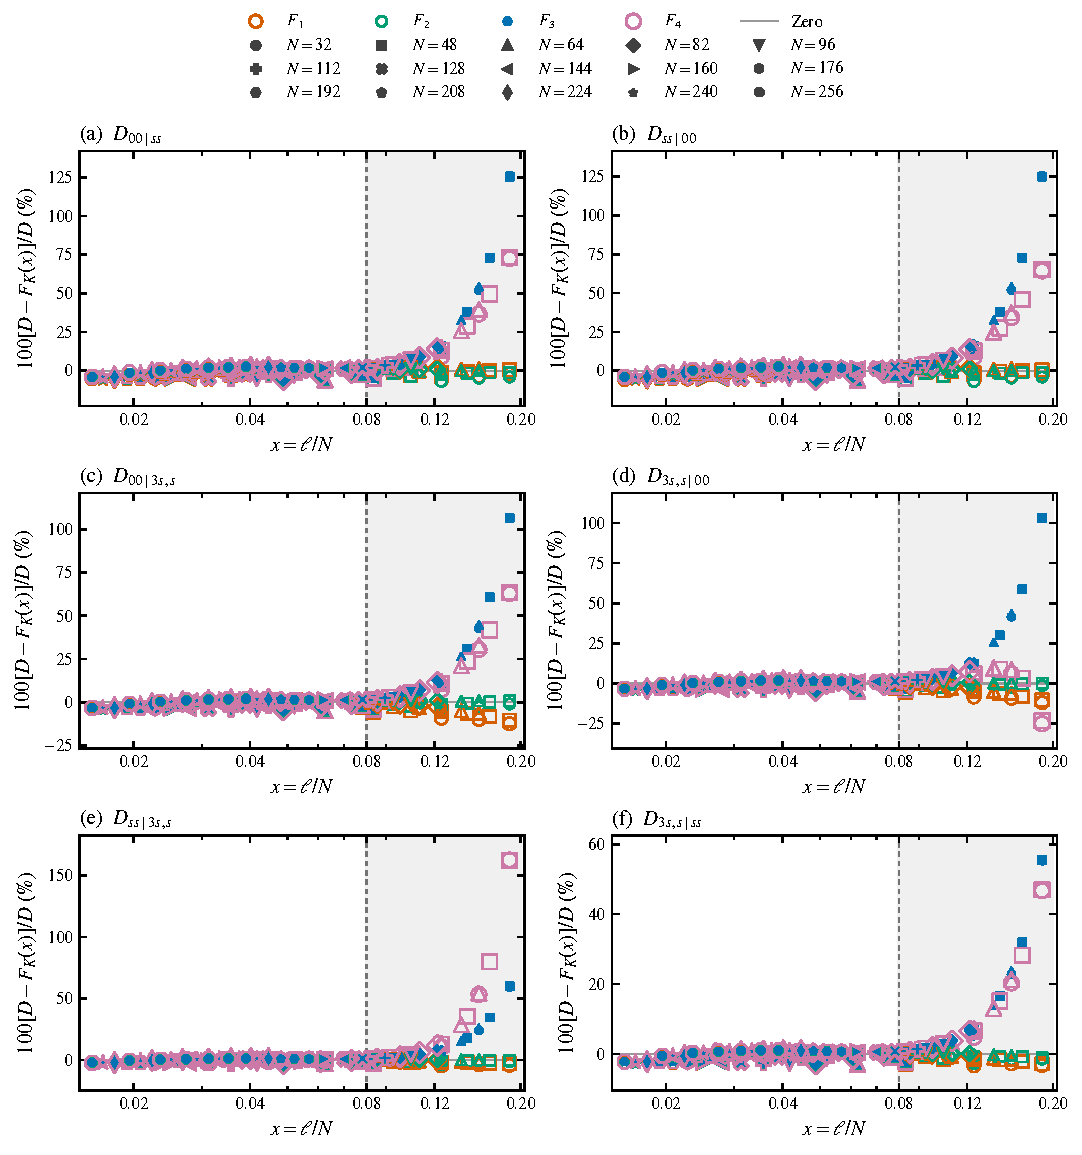
\includegraphics[width=.95\linewidth]{../figs/boson_residuals.pdf}
\caption{Boson residual comparison for the parameters, geometries,
and fit functions of Fig.~\ref{fig:bosonfits}. The ordinate is
$100[y_i-F_K(x_i)]/y_i$, where $y_i$ is the numerical directed relative
entropy and $K=1,2,3,4$. Open orange, open green, filled blue, and open
purple markers denote $F_1,F_2,F_3,F_4$, respectively. Marker shape
identifies $N$; marker sizes distinguish overlaps, and the gray line
marks zero. All fits use the same 77 samples with $x\leq0.08$, $p=1/2$, fixed powers
$2,4,\ldots,2K$, and $K$ free coefficients optimized by unweighted
least squares in $D$. All 100 displayed points are shown, including the
23 outside-fit points in the shaded region $0.08<x\leq0.20$.
The vertical scale is linear throughout, with ticks showing the signed
percentage values directly; $x$ is logarithmic. Complete results are in Appendix~\ref{sec:allfits}.
Persistent separation of points with nearby or
identical $x$ indicates limitations of describing these finite-chain
data by a function of $x$ alone.}
\label{fig:bosonresid}
\end{figure}
\clearpage
